% Generated Bauer double-ladder figure bundle; include manually from main.tex.
\begin{figure*}[!tbp]
  \centering
  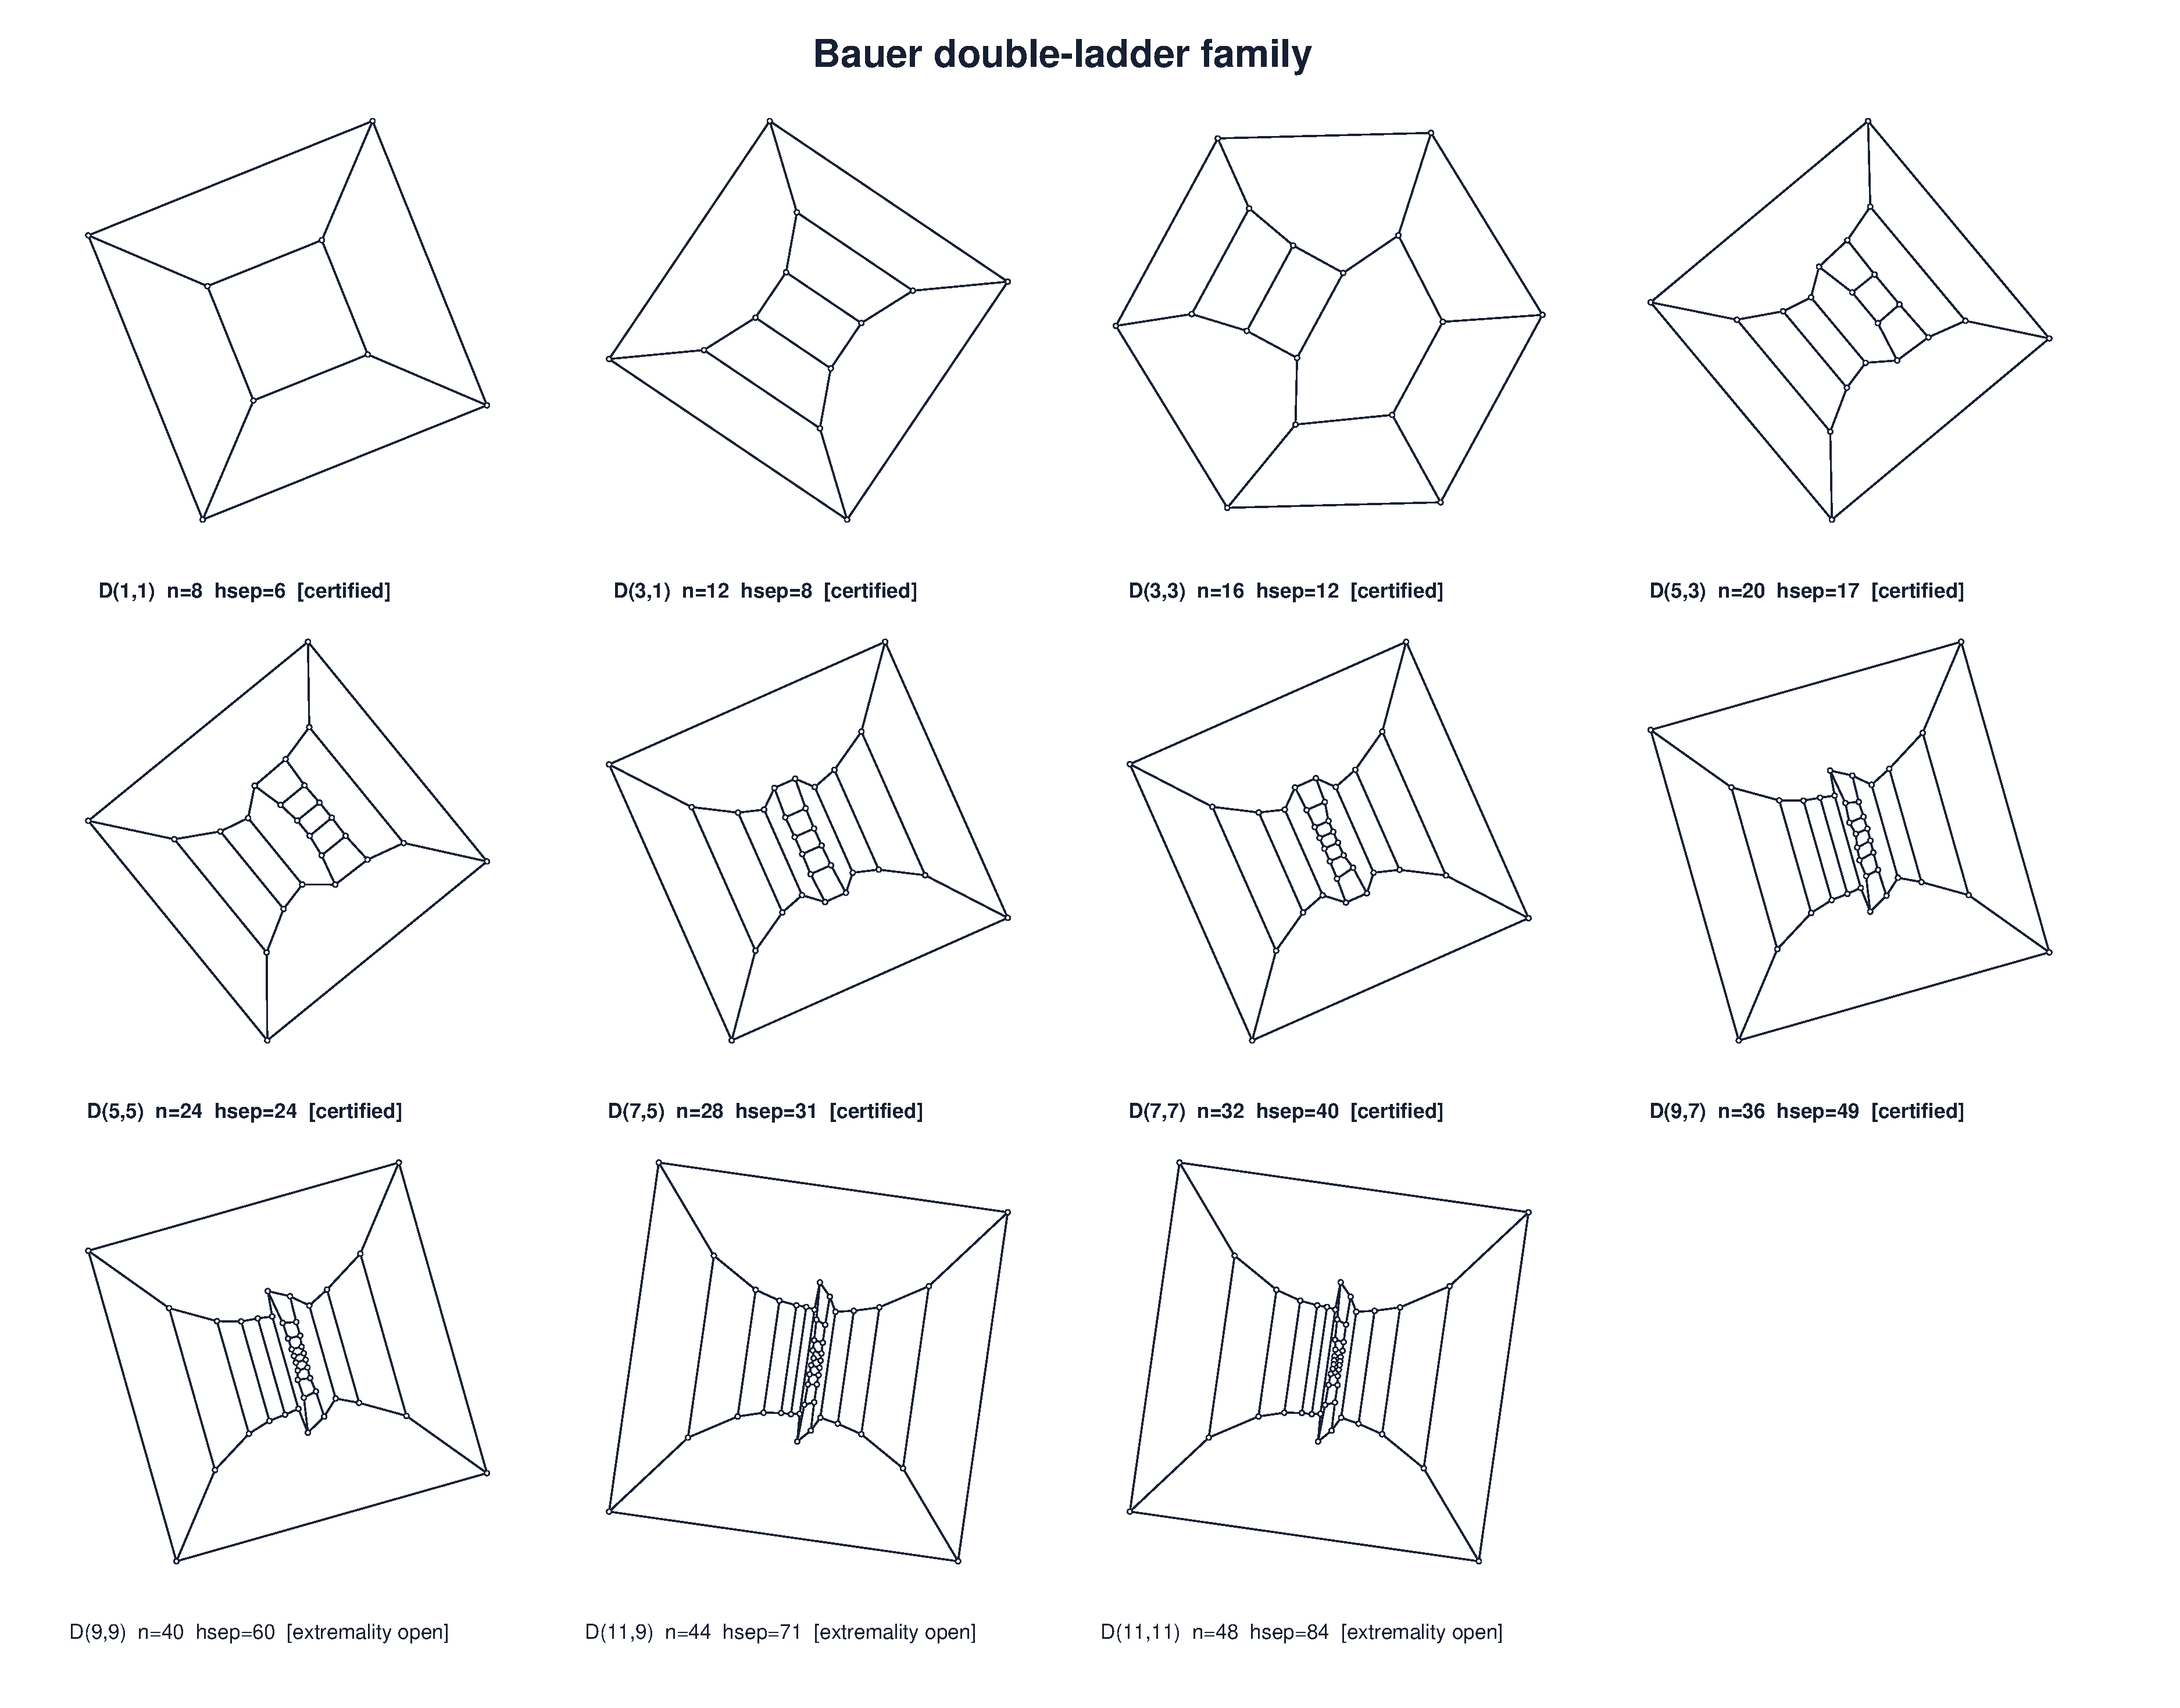
\includegraphics[width=.98\textwidth]{figures/bauer_family/complete_family.pdf}
  \caption{The Bauer double-ladder family from $D(1,1)$ through $D(11,11)$. Open-order members at orders 40, 44, and 48 have exact graph-specific certificates but no complete-census extremality claim.}
  \label{fig:bauer-complete-family}
\end{figure*}

\begin{figure*}[!tbp]
  \centering
  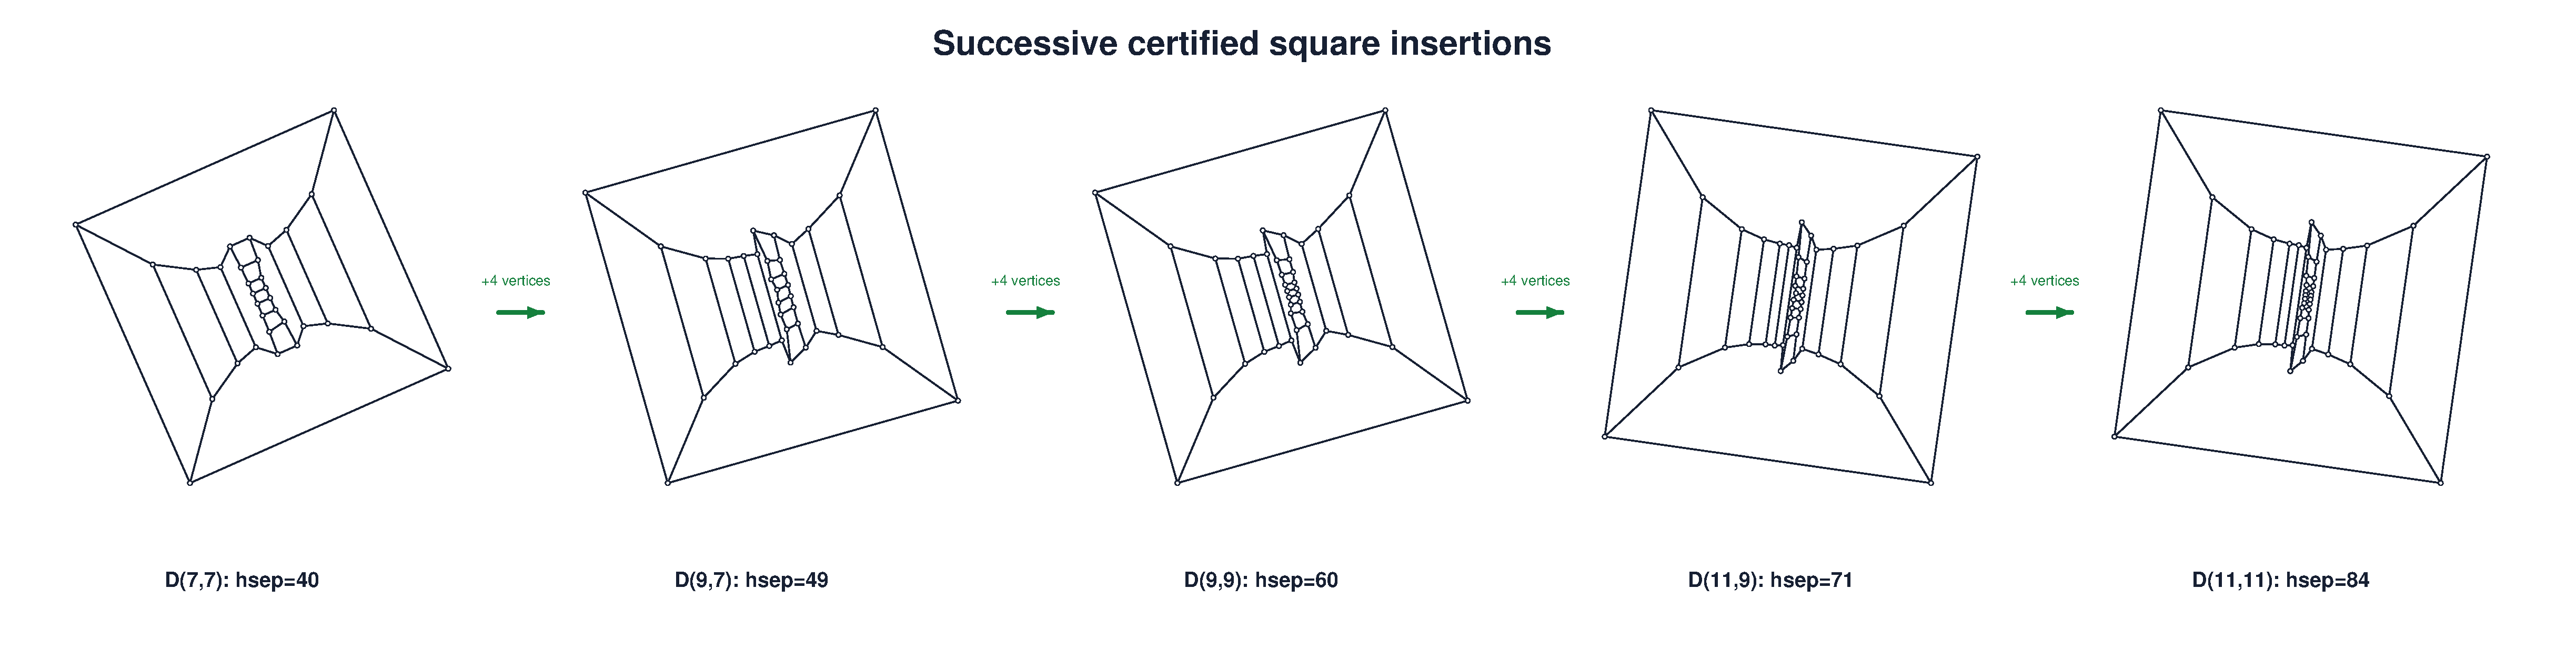
\includegraphics[width=.98\textwidth]{figures/bauer_family/insertion_sequence.pdf}
  \caption{Successive certified facial square insertions from $D(7,7)$ to $D(11,11)$.}
  \label{fig:bauer-insertion-sequence}
\end{figure*}

\begin{figure*}[!tbp]
  \centering
  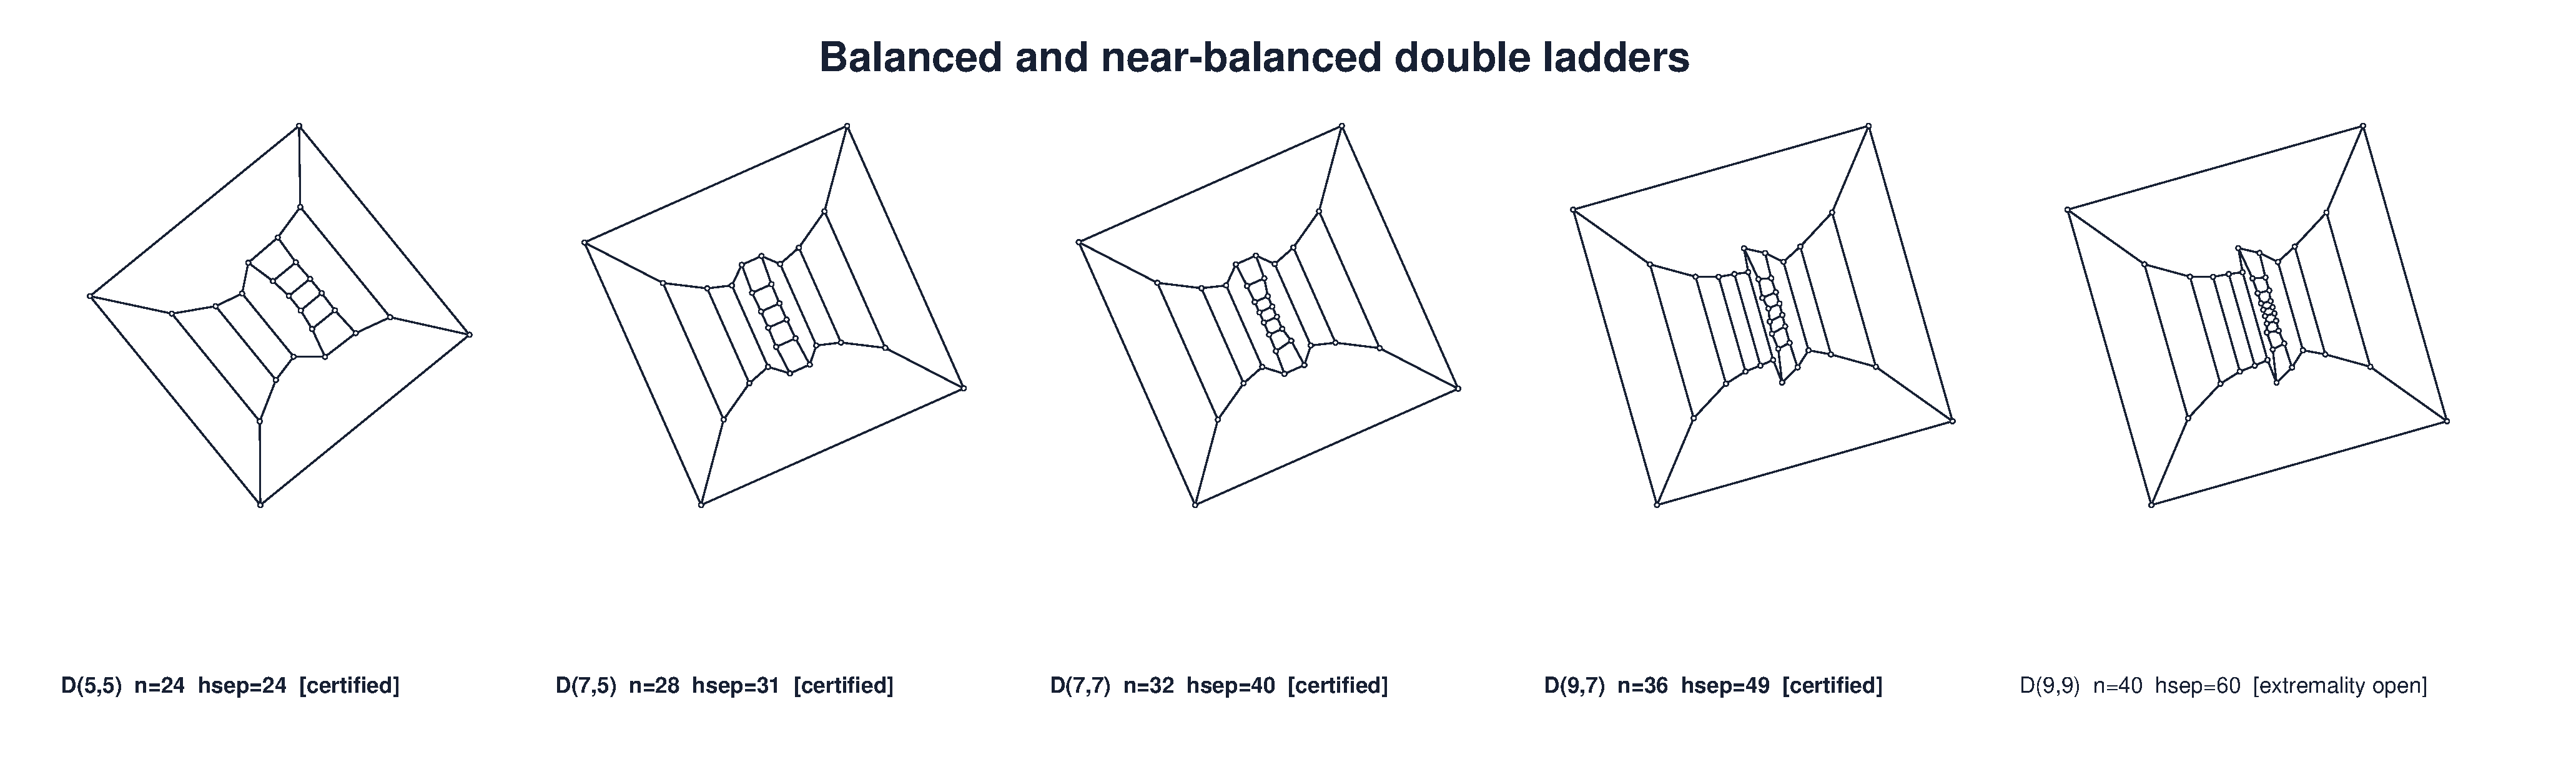
\includegraphics[width=.98\textwidth]{figures/bauer_family/balance_comparison.pdf}
  \caption{Balanced and near-balanced double ladders, with the two ladder parameters shown in common orientation.}
  \label{fig:bauer-balance}
\end{figure*}

\begin{figure}[!tbp]
  \centering
  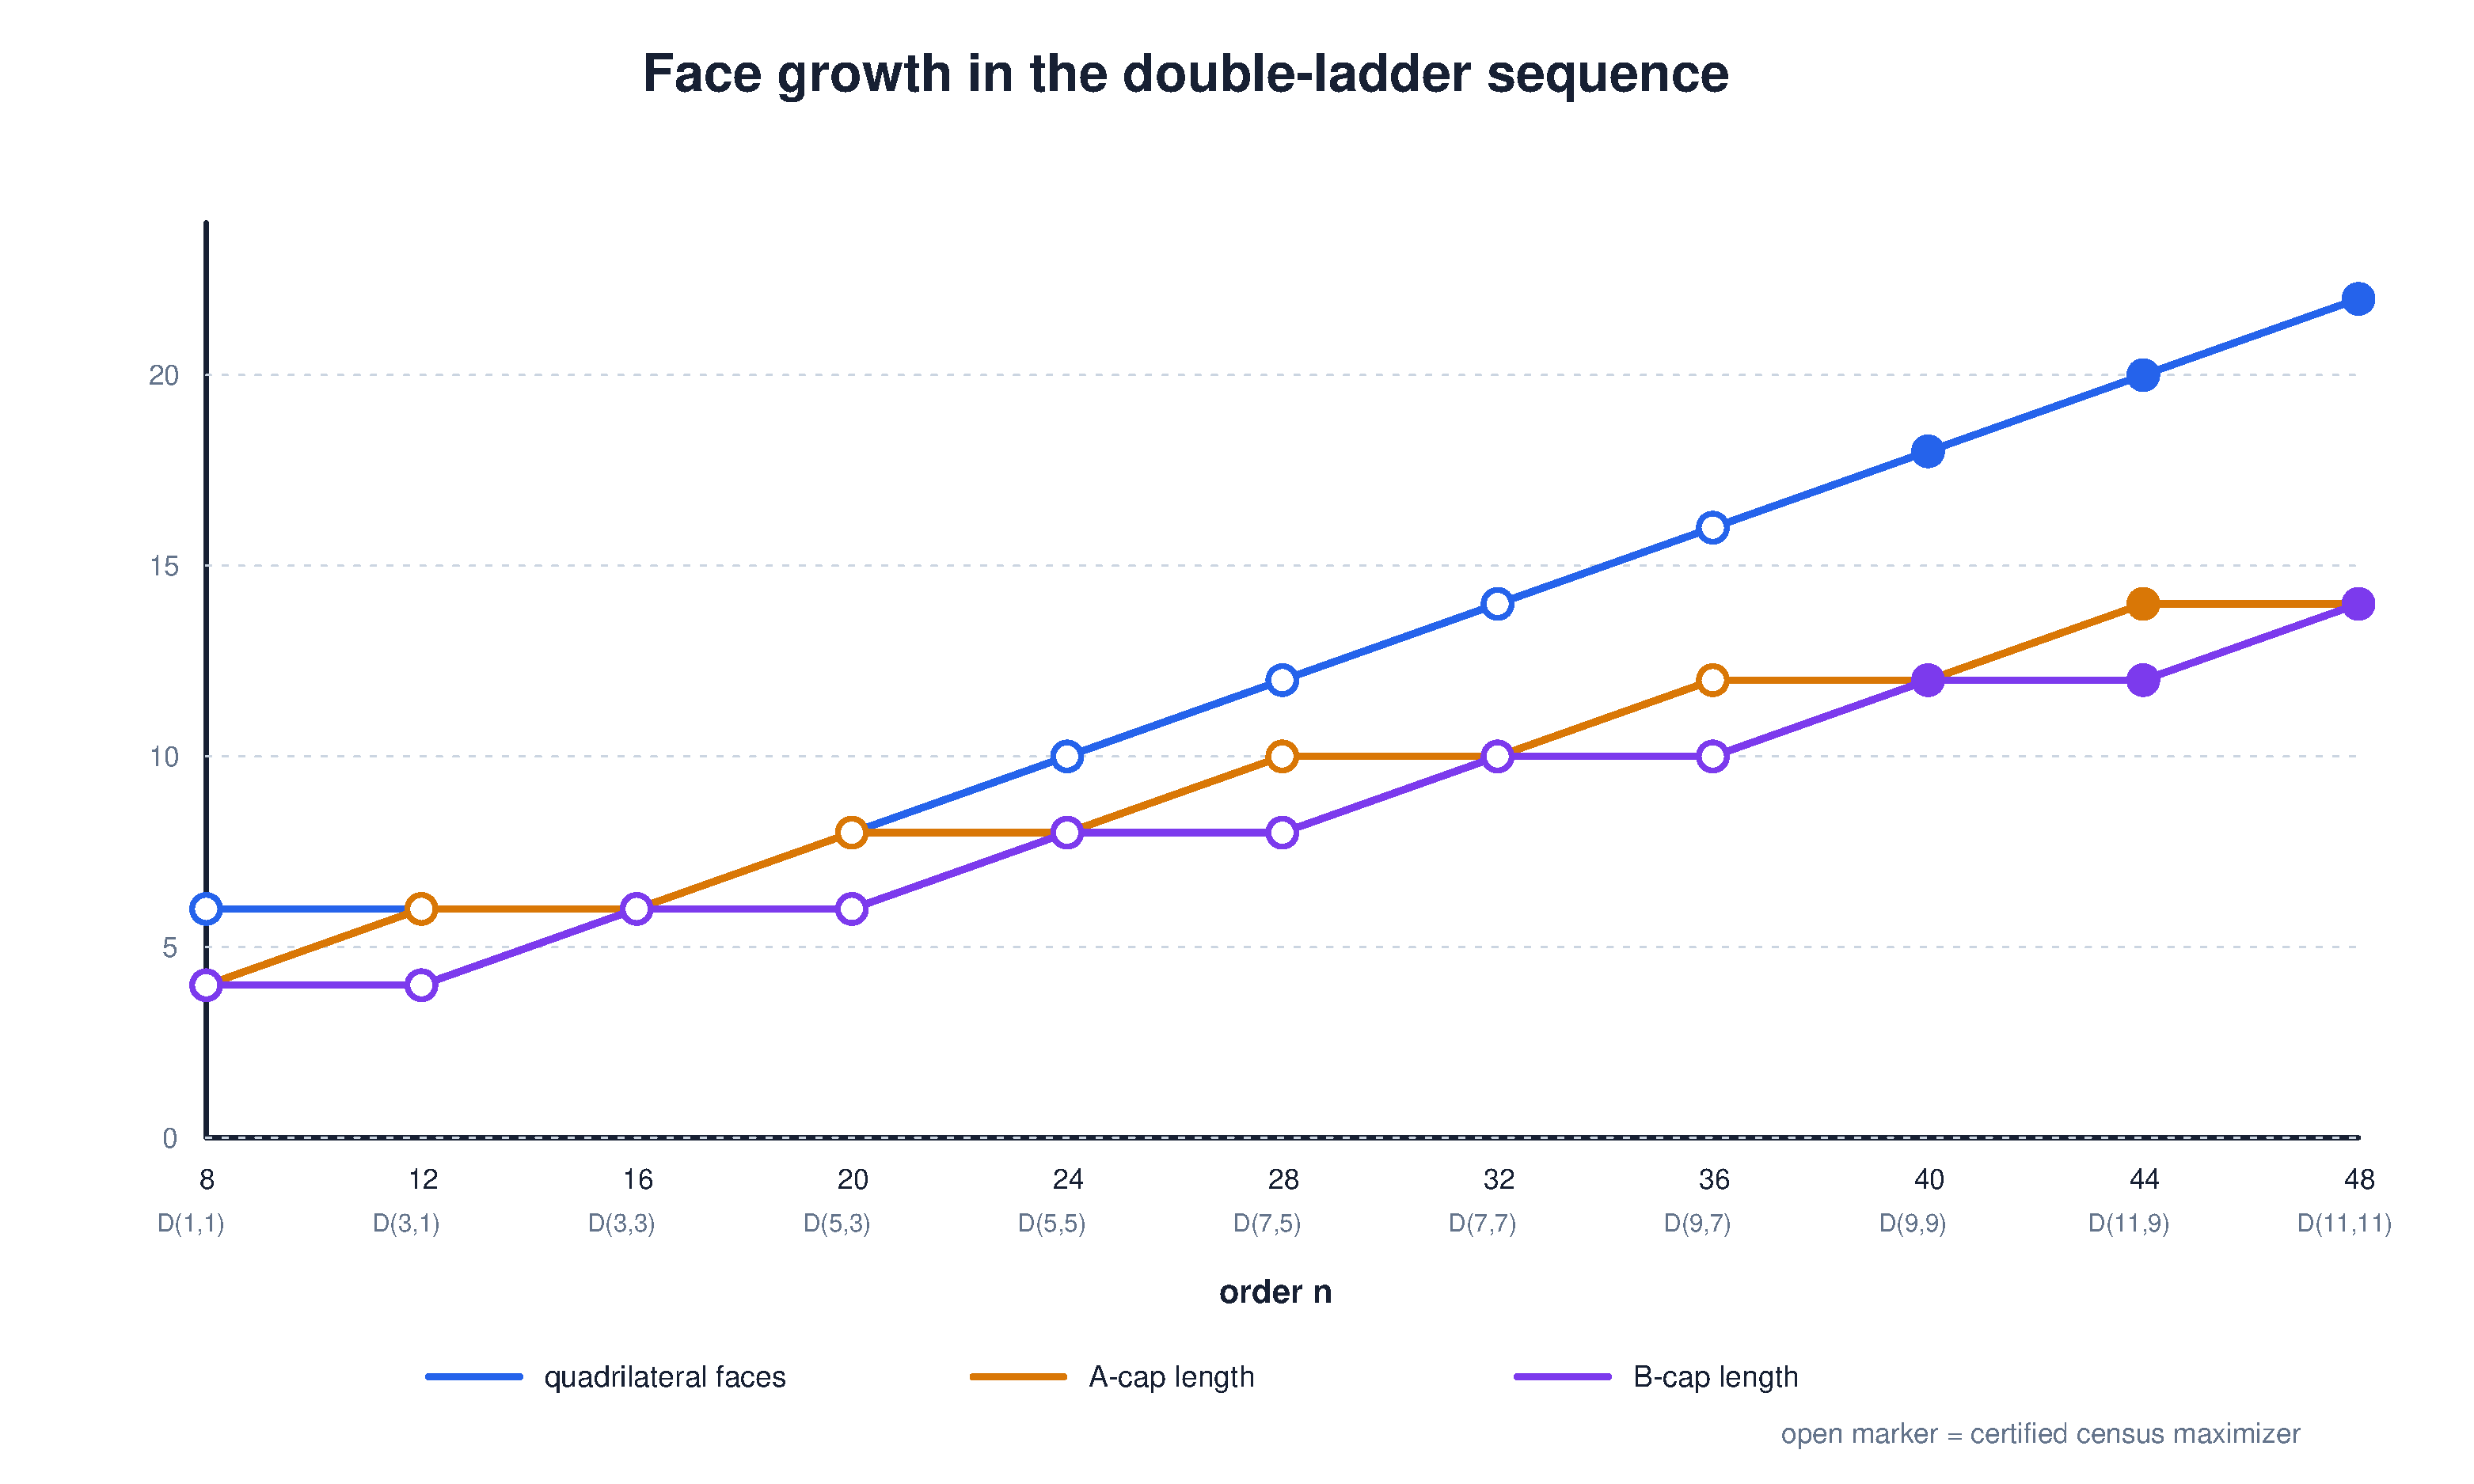
\includegraphics[width=.98\linewidth]{figures/bauer_family/face_growth.pdf}
  \caption{Growth of quadrilateral cells and cap-face lengths in the displayed family.}
  \label{fig:bauer-face-growth}
\end{figure}

\begin{figure}[!tbp]
  \centering
  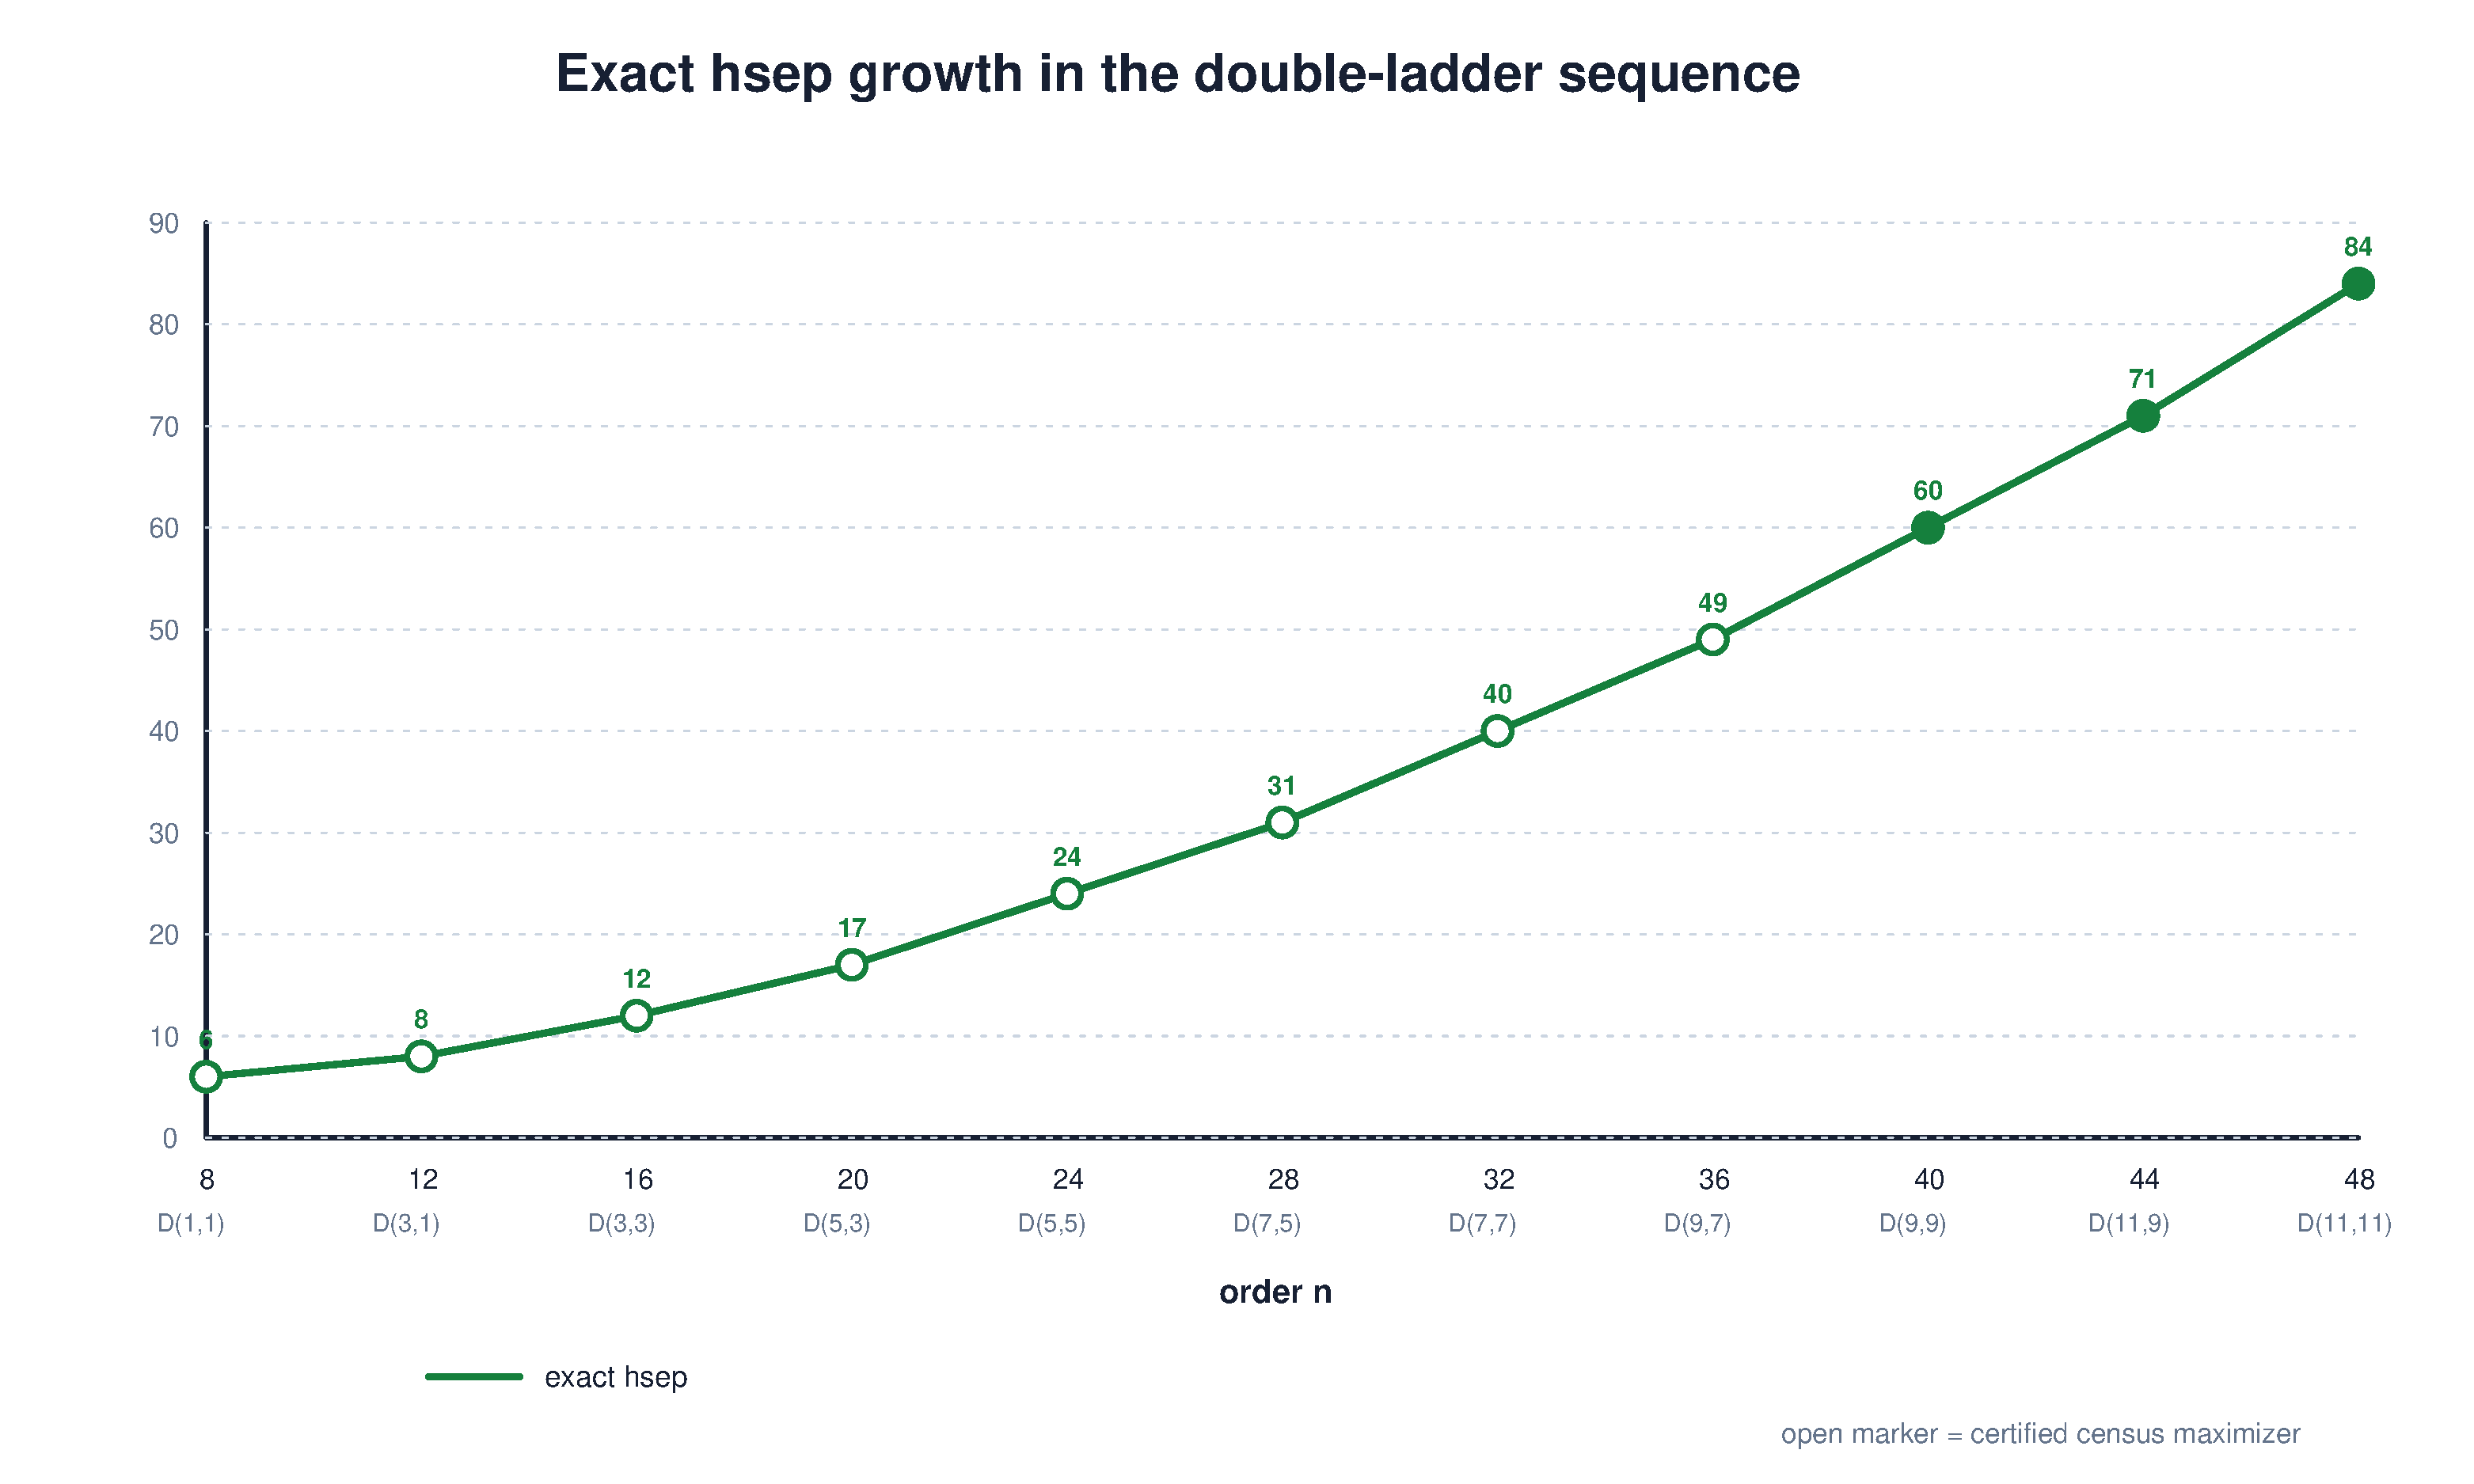
\includegraphics[width=.98\linewidth]{figures/bauer_family/hsep_growth.pdf}
  \caption{Certified exact $\operatorname{hsep}$ values along the displayed family. Filled markers denote graph-specific results beyond the completed order-36 census.}
  \label{fig:bauer-hsep-growth}
\end{figure}
